%------------------------------début entêtes-----------------------------------------
\pagestyle{fancy}

\renewcommand{\footrulewidth}{1pt}

\fancyhead[L]{État de l'art}
\fancyhead[C]{\thepage}
\fancyhead[R]{Génération de descriptions}

\fancyfoot[L]{Ny Hoavy Nomena}
\fancyfoot[C]{\thepage}
\fancyfoot[R]{Annotation automatique d'images}

%------------------------------fin entêtes-------------------------------------------

\subsection{Génération automatique de descriptions d'images} \label{associationit}
\qquad Cette partie du rapport s'intéresse aux modèles multimodaux  pour l'appariement de texte et images et à la génération automatique de descriptions.\\
Présenté  dans les sections précédentes, l'apprentissage profond est un outil performant dans le domaine de la vision par ordinateur et le TALN. Les modèles de génération automatique de descriptions étudiés combinent ces méthodes pour analyser d'un côté les images et de l'autre les textes afin de les associer.\\
En général, les modèles analysent les propriétés statistiques de chaque modalité (texte et image) de la base de données d'apprentissage. Ces méthodes ont pour objectif de projeter les caractéristiques visuelles et textuelles dans un même espace (espace d'intégration ou espace sémantique). Ces systèmes sont utilisés à la fois pour la rechercher des textes associés à une image et vice-versa (figure \ref{fig:multimodal}). Pendant l'apprentissage, les images et textes sont projetés dans l'espace d'intégration de telle sorte que les plus proches voisins ont des significations assez similaires.\\

\begin{figure}[h]
	\begin{center}
		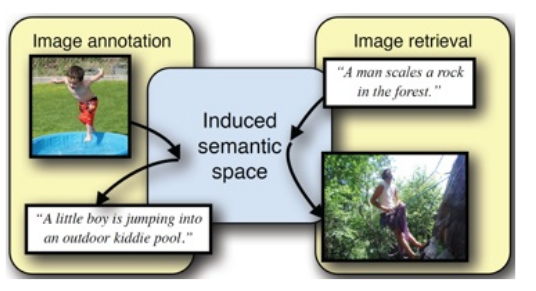
\includegraphics[width=0.4\textwidth]{multimodalArticle}
		\caption{Illustration des systèmes mutlimodaux pour l'annotation et la recherche d'images \cite{bernardi2016automatic} \label{fig:multimodal}}
	\end{center}
\end{figure}

L'ACC (Analyse Canonique de corrélation) a été utilisée dans nombreuses études pour explorer les relations pouvant exister entre deux variables aléatoires de dimension différente (littérature ACC on parle de vue). Dans notre étude les deux variables correspondent aux vecteurs caractéristiques des deux modalités. Le but de l'ACC est de trouver 2 vecteurs de projections $w_{x}$ et $w_{y}$ tels que la corrélation entre la projection des 2 variables $ X \in \mathbb{R}^{m\times p}$ et $Y \in \mathbb{R}^{m\times q}$ (d'un échantillon de taille $m$) soit maximisée. Ces 2 vecteurs de projections $w_{x}$ et $w_{y}$ sont calculés par maximisation du coefficient de corrélation $\rho$ qui se réduit par :\\
\begin{eqnarray}
\rho = \operatorname*{arg\,max}_{w_{x},w_{y}} \frac{w^{T}_{x}XY w_{y}}{\sqrt{(w^{T}_{x}XX^{T}w_{x}) (w^{T}_{y}YY^{T}w_{y})}}
\end{eqnarray}	
%Plusieurs vecteurs de projection peuvent être retrouvés ce qui va former une matrice de projection :$W_{x} \in \mathbb{R}^{p\times l}$ et de même $W_{y} \in \mathbb{R}^{q\times l}$. $l \leq \min(p,q)$
%Cette équation va se réduire en un problème de vecteurs propres détaillés dans \cite{hardoon2004canonical}

Les vecteurs de projection maximisant le coefficient de corrélation $rho$  sont  alors utilisés pour projeter les vecteurs des 2 vues afin de les comparer.\\
%Soient :\\
%$U$ la projection des vecteurs descripteurs des images : $U=(X-\mu X)w_{x}$
%$V$ la projection des vecteurs caractéristiques des labels : $V=(Y-\mu Y)w_{y}$
%	Pour l'annotation d'une image, le vecteur descripteur de l'image $xt$ est projeté dans l'espace d'intégration à partir du vecteur de projection correspondant ($w_{x}$) : $ut = (x_{t}-\mu X)$ pour ensuite calculer la distance de corrélation aux projections des labels $V$. Le label qui correspond à la plus proche (en considérant la distance de corrélation) $V_{i}$ est assigné à l'image. 
Cette méthode a été utilisée par \cite{murthy2015automatic} pour l'annotation des images par des labels. Dans leur article, des variations de l'ACC ont été aussi étudiée à savoir  Kernel CCA. Le Kernel CCA se différencie de ACC par la projection  des variables dans un espace de grande dimension appelé : espace de redescription [kernel trick], une transformation non-linéaire pour exploiter des relations non-linéaires entre les variables. Les vecteurs caractéristiques $X$ de l'image et $Y$ des labels ou étiquettes ont été respectivement extraits grâce à un réseau de neurones convolutif pré-entrainé d'Oxford (VGG) et le modèle skip-gram pré-entrainé de Mikolov et al. Word2Vec \cite{mikolov2013efficient}. \cite{gong2014improving}  \cite{gong2014multi}  a montré qu'une normalisation appropriée améliore l'ACC linéaire sur une grande collection de données.
L'apprentissage profond intervient dans l'ACC en proposant le Deep CCA \cite{mikolajczyk2015deep}. L'efficacité de l'apprentissage profond à maximiser la corrélation définie par l'ACC a été démontrée et ceci par apprentissage bout à bout à travers un réseau de neurones par rétropropagation.
\medskip
%\begin{figure}[h]
%	\begin{center}
%		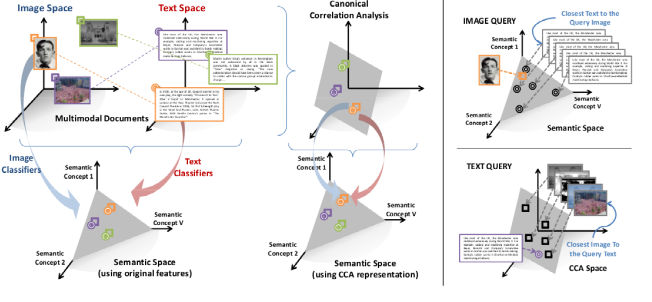
\includegraphics[width=0.4\textwidth]{cca}
%		\caption{Illustration de l'approche basée sur l'ACC pour un système de recherche multimodale \cite{rasiwasia2010new}}
%	\end{center}
%\end{figure}
\\

A part l'utilisation de l'ACC les modèles profonds traitent le problème par apprentissage profond de la similarité. Les paramètres de projection de différentes modalités sont calculés par apprentissage d'un RNA en optimisant une fonction objectif convenable à l'appariement des modalités dans l'espace sémantique. Ces modèles sont entraînés par rétropropagation des erreurs et  s'adaptent facilement à de grandes quantités de données.\\
%En general, la fonction objectif \textbf{apparie} les images et textes en maximisant les scores entre textes et images qui se correspondent. 

	\textit{DeViSE} : Deep Visual-Semantic Emedding est un modèle créé par Andrea Frome et al. \cite{frome2013devise} pour la classification d'images sur beaucoup de catégories. \textit{DeViSE} utilise les textes associés à l'image pour améliorer les systèmes de classification existants.  La contribution majeure de ce modèle est l'apprentissage des réseaux de neurones convolutifs à prédire les vecteurs caractéristiques textuels des labels associés à l'image en entrée. Pour cela Andrea Frome et al. ont pré-entrainé un réseau de neurones convolutifs pour la reconnaissance d'objets basé sur l'architecture d'AlexNet. Les labels associés à chaque image sont représentés par le vecteur représentatif issu des méthodes de  word embedding à partir du modèle de Mikolov et al. entrainé sur 5.7 millions de documents (5.4 billion mots) issus du wikipedia.org. Le réseau de neurones convolutifs pré-entrainé a été ensuite modifié pour prédire les vecteurs caractéristiques de chaque texte associé aux images par apprentissage en optimisant la fonction objectif à marge suivante :
\begin{eqnarray}
	cout(image,label)= \sum_{j \neq label} max[0,marge- \vec{t}_{label}M \vec{v}(image)+ \vec{t}_{j}M \vec{v}(image)]
\end{eqnarray}\\
$\vec{v}(image)$ est le vecteur caractéristique de l'image en entrée\\
$M$ est la matrice des paramètres.\\
$\vec{t}_{label}$ est le vecteur caractéristique du label associé à l'image\\
Les $\vec{t}_{j}$ sont les vecteurs caractéristiques des autres labels.\\
Cette approche a permis à ce modèle de classifier des images appartenant à d'autres catégories auxquelles le modèle n'a pas été entraîné. Cela est dû, en majeure partie, à l'utilisation des vecteurs caractéristiques issus du skip-gram modèle de Mirkov et al.\\
Plusieurs travaux s'inspirent de DeViSE pour créer des modèles pour associer image et texte.\\

Certains travaux ont proposé des fonctions objectifs plus intéressantes : les fonctions objectifs bidirectionnelles (bidirectional ranking loss). En plus d'encourager l'attribution de scores supérieurs aux phrases décrivant l'image, ces fonctions assurent pour chaque phrase que: les images qu'elle décrit aient des scores supérieurs à ceux des images décrites par les autres. \\

Dans \cite{karpathy2015deep} et \cite{karpathy2014deep} Andrej Karpathy et Li Fei-Fei ont défini une fonction objectif structurée pour aligner des fragments d'image (régions de l'image) et des fragments de texte (groupe de mots) pour générer des descriptions pour chaque région pertinente de l'image. Cette fonction objectif entraîne le modèle pour que les scores obtenus par les images et textes correspondants aient des scores largement supérieurs (à l'aide d'une marge) à ceux qui ne se correspondent pas (bidirectionnelle). Le score obtenu à partir d'une image $k$ et d'une phrase $l$ est donné par l'équation \ref{eq:score}.
\begin{eqnarray}
\label{eq:score}
S_{kl}=\sum_{t\in g_{k}} \sum_{i\in g_{k}}max(0,v^{T}_{i} s_{t})
\end{eqnarray}
$g_{k}$ est l'ensemble des fragments de l'image $k$ et $ g_{l}$ l'ensemble des fragments du texte $l$.\\
$ v^{T}_{i} s_{t}$ est le produit scalaire, interprété comme étant la mesure de similarité entre le i-ème région de l'image et le t-ème mot de la phrase.\\
$v_{i}$ : projection du vecteur caractéristique de l'i-ème région de l'image.\\ Les régions ont été extraites à partir d'un modèle de réseau neuronal convolutif utilisé dans la détection d'objets \cite{jitendramalikrich} pré-entrainé sur ImageNet et affiné pour la détection de 200 classes d'ImageNet Detection Challenge \cite{russakovsky2015imagenet}.\\
$s_{t}$ : est la projection du vecteur caractéristique du t-éme mot dans  le modèle de langue \cite{karpathy2015deep} \cite{karpathy2014deep}. \\

Ainsi tous les mots $s_{t}$ sont alignés par la meilleure région de l'image. En considérant que $k=l$ désigne la correspondance entre l'image et la phrase, la fonction objectif structurée finale est définie par :
\begin{eqnarray}
C(\theta)= \sum_{k}[\sum_{l}max(0,S_{kl}-S_{kk}+1)+\sum_{l}max(0,S_{lk}-S_{kk}+1)]
\end{eqnarray}

\qquad	De même, pour l'apprentissage de leur modèle, Ryan Kiros et al. \cite{kiros2014unifying} ont minimisé la fonction objectif bidirectionnelle suivante pour apparier les phrases et images qui se correspondent.\\
\begin{eqnarray}
C(\theta)= \sum_{x}[\sum_{k}max(0,\alpha - s(x,v)+ s(x,v_k) + \sum_{v} \sum_{k} max(0,\alpha - s(v,x)+s(v,x_k))].
\end{eqnarray}
$s(a,b) = a.b$ est le produit scalaire entre le vecteur $a$ et $b$\\
$v_k$  sont les vecteurs caractéristiques des phrases qui ne correspondent pas (ne décrivent pas) l'image $x$.\\
$x_k$ sont les images qui ne sont pas décrites par $v$.\\
$\alpha$ : est la marge (=1 pour les méthodes citées dans \cite{karpathy2015deep} et \cite{karpathy2014deep})


\qquad Récemment, les travaux de recherche s'intéressent à la génération de descriptions d'images par des phrases : \textit{"image captionning"} en anglais. Les modèles pour la génération de phrases descriptives suivants appliquent le principe de l'autoencodeur : encodeur-décodeur, issus des systèmes de traduction neuronaux (Neural Machine Translation), sur les images et les phrases associées. Dans ce cas, l'encodeur concerne  l'analyse et la représentation des images et le décodeur  génère la séquence de mots pour décrire l'image. En se référant à la génération de phrases dans les travaux de TALN (section \ref{phrasegen}) et à la représentation des images dans la vision par ordinateur (section \ref{vo}), les modèles de génération de descriptions  sont composés de réseaux de neurones convolutifs pour encoder l'image et de réseaux de neurones récurrents comme modèle de langue pour décoder.\\
\qquad	En considérant l'image $I$, on définie la loi de probabilité à estimer :
$P(w_{1:L}| I)$ dont $w_{1:L}$ : la séquence de mots de longueur $L$.
Pour la génération de la séquence, le modèle de langue estime la loi de probabilité $P(w_i| w{1:i-1}, I)$ qui représente la probabilité de générer un mot $w_i$ sachant la séquence de mots observée $w_{1:i-1}$ et l'image $I$. 

La figure [figure \ref{cnnlstm}] illustre l'architecture générale des modèles de génération de descriptions d'une image.\\
\medskip
\begin{figure}[h]
	\begin{center}
		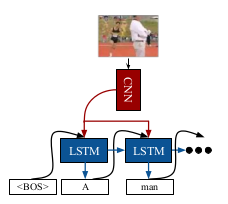
\includegraphics[width=0.4\textwidth]{cnnlstm}
		\caption{Illustration du modèle CNN-LSTM pour la génération de phrases décrivant l'image \cite{donahue2015long} \label{cnnlstm}}
	\end{center}
\end{figure}

Le réseau de neurones convolutifs fournit la caractéristique visuelle de l'image tandis que le modèle de langue est entraîné pour prédire chaque mot de la phrase descriptive donnée par la probabilité $P(w_i| w{1:i-1}, I)$.

\qquad	La principale contribution de ces modèles de description d'images s'intéresse à la manière de combiner l'information visuelle (issus du réseau de neurones convolutifs), textuelle (grâce aux méthodes de \textit{"word embedding "}) et le contexte (stocké par le réseau de neurones récurrents) pour générer la séquence de mots qui décrit l'image.

\qquad	LRCN \cite{donahue2015long} est un modèle CNN-LSTM créé pour les tâches de la vision par ordinateur impliquant un traitement de séquences de données : reconnaissance d'activité, description d'une image et vidéos. Pour la génération de descriptions d'images LRCN propose 3 variations ($LRCN_{1u}$, $LRCN_{2u}$, $LRCN_{2f}$) de son modèle se basant sur le nombre de couches LSTM et l'introduction de l'information visuelle.
$LRCN_{1u}$ et $LRCN_{2u}$  sont composés respectivement d'une seule couche et de deux couches de LSTM. Dans ces deux modèles, le vecteur caractéristique visuel est concaténé avec la représentation textuelle et imbriqué dans le premier LSTM de l'empilement. Tandis que pour $LRCN_{2f}$ (composé de deux couches) le vecteur caractéristique visuelle est concaténé avec l'état caché précédent avant d'être introduit dans le LSTM de la couche courante. Avec les mêmes configurations, $LRCN_{2f}$ a obtenu la meilleure performance sur les trois modèles pour son architecture.\\

\qquad	Dans \cite{karpathy2015deep} \cite{vinyals2015show}, le modèle de génération de descriptions est basé sur un RNN multimodal.
Le réseau de neurones récurrents génère une séquence de mots en relation avec l'image en initialisant sa couche cachée par le vecteur caractéristique visuel.
Le RNN prend en entrée le vecteur caractéristique visuel une seule fois à l'instant $t=1$ pour \cite{karpathy2015deep} et $t=-1$ dans \cite{vinyals2015show}.
Le RNN multimodal est definie par :\\
\begin{eqnarray} 
b_v = W_{hi}[CNN_{\theta_c}(I)]\\
h_t = f(W_{hx} x_t + W_{hh} h_{t-1}+b_h+ \mathbbm{1}(t=i) \odot b_v)\\
y_t = softmax(W_{oh} h_t+b_o).
\end{eqnarray}\\
$CNN_{\theta_c}(I)$: est le vecteur caractéristique de l'image $I$ issus de la dernière couche d'un réseau de neurones convolutifs.\\
$x_t$: est le vecteur représentatif du mot à l'instant t.\\
$\mathbbm{1}$ est une fonction indicatrice\\
$\mathbbm{1}(t=i)$: indique l'instant auquel le vecteur caractéristique de l'image $I$ représenté par $b_v$ est injecté. \\
$i=-1$ pour \cite{vinyals2015show}\\
$i=1$ pour \cite{karpathy2015deep}